%\title{CS4221/CS5421 Database Applications Design and Tuning}
\title{CS4221/CS5421}

\subtitle{Tutorial 3: Dependency}

\author{Mark Meng Huasong}

\institute[National University of Singapore] % (optional, but mostly needed)
{
	School of Computing\\
	National University of Singapore
}

\titlegraphic{
	
\includegraphics[width=2cm]{nus-logo}
}

\date{Week 5, 2022 Spring}

\begin{frame}
	\titlepage
	\begin{tcolorbox}
		\begin{center}
			{\scriptsize \textcolor{red}{All the materials within presentation slides are protected by copyrights.\\
					It is forbidden by NUS to upload these materials to the Internet.}}
		\end{center}
	\end{tcolorbox}
\end{frame}

\begin{frame}
	Updated on 12 Feb (Saturday):
	\begin{itemize}
		\item Added some notes regarding finding all minimal covers on page 10 and 12.
	\end{itemize}
\end{frame}

\begin{comment}
\section*{Greeting!}
\begin{frame}[fragile]{Greeting!}
	Welcome to CS5221/CS5421!\vspace{15pt}
	
	\textbf{Mark MENG Huasong} (
\includegraphics[height=\fontcharht\font`\B]{t1/images/chn-chars.png}) \vspace{15pt}
	
	B.Eng.(Hons), Computer Science, Nanyang Technological University
	
	M.Comp., Infocomm Security, National University of Singapore\vspace{15pt}
	
	Been in cyber-security R\&D industry since 2014, came back NUS for PhD in 2019\vspace{15pt}
	
	I will be your TA for the remaining of this semester!
\end{frame}
\end{comment}

\section*{Question 1 Functional Dependencies}

\begin{frame}[fragile]{Question 1}
Consider the relational schema $R=\{A, B, C, D, E\}$ with the following set of functional dependencies.\\\vspace{5pt}
$\Sigma=\{\{A, B\} \rightarrow \{C\}, \{D\} \rightarrow \{D, B\}, \{B\} \rightarrow \{E\}, \{E\} \rightarrow \{D\}, \{A, B, D\} \rightarrow \{A, B, C, D\}\}$.
\end{frame}

\begin{frame}[fragile]{Question 1 (a-b) Attribute Closure \& Candidate Keys}
\textbf{(a) Compute all the closures of the the sets of attributes that are not equal to themselves, are not super-keys or are candidate keys.} \\
\textbf{What information is not essential and could be removed.}\vspace{15pt}

\textbf{Solution}: \vspace{3pt}

\begin{columns}[t]
	\column{0.45\textwidth}
	\textcolor{gray}{\scriptsize \textit{(Let's start with single attribute first)}}\\
	\textcolor{gray}{$\{A\}^{+}= \{A\}$ \scriptsize \textit{(omitted)}}\\	
	$\{B\}^{+}= \{B, D, E\}$\\	
	\textcolor{gray}{$\{C\}^{+}= \{C\}$ \scriptsize \textit{(omitted)}}\\
	$\{D\}^{+}= \{B, D, E\}$\\
	$\{E\}^{+}= \{B, D, E\}$\\ \vspace{5pt}
	\textcolor{gray}{\textit{\scriptsize (Two attributes' combination)}}\\
	$\underline{\{A, B\}^{+}}= \{A, B, C, D, E\}$\\
	\textcolor{gray}{$\{A, C\}^{+}= \{A, C\}$ \scriptsize \textit{(omitted)}}\\
	$\underline{\{A, D\}^{+}}= \{A, B, C, D, E\}$\\
	$\underline{\{A, E\}^{+}}= \{A, B, C, D, E\}$
	\column{0.45\textwidth}	
	$\{B, C\}^{+}= \{B, C, D, E\}$\\
	$\{B, D\}^{+}= \{B, D, E\}$\\
	$\{B, E\}^{+}= \{B, D, E\}$\\
	$\{C, D\}^{+}= \{B, C, D, E\}$\\
	$\{C, E\}^{+}= \{B, C, D, E\}$\\
	$\{D, E\}^{+}= \{B, D, E\}$\\
	 \vspace{5pt}
	Other attribute closures need not be computed.
\end{columns}
\end{frame}

\begin{frame}[fragile]{Question 1 (a-b) Cont.}
	We see the candidate keys are $\{A,B\}$, $\{A,D\}$ and $\{A,E\}$.\\
	\textcolor{blue}{This is the answer for 1(b)}\\
	\vspace{15pt}
	\textit{We can also visualize the FD as a figure below:}\\
	\begin{figure}
		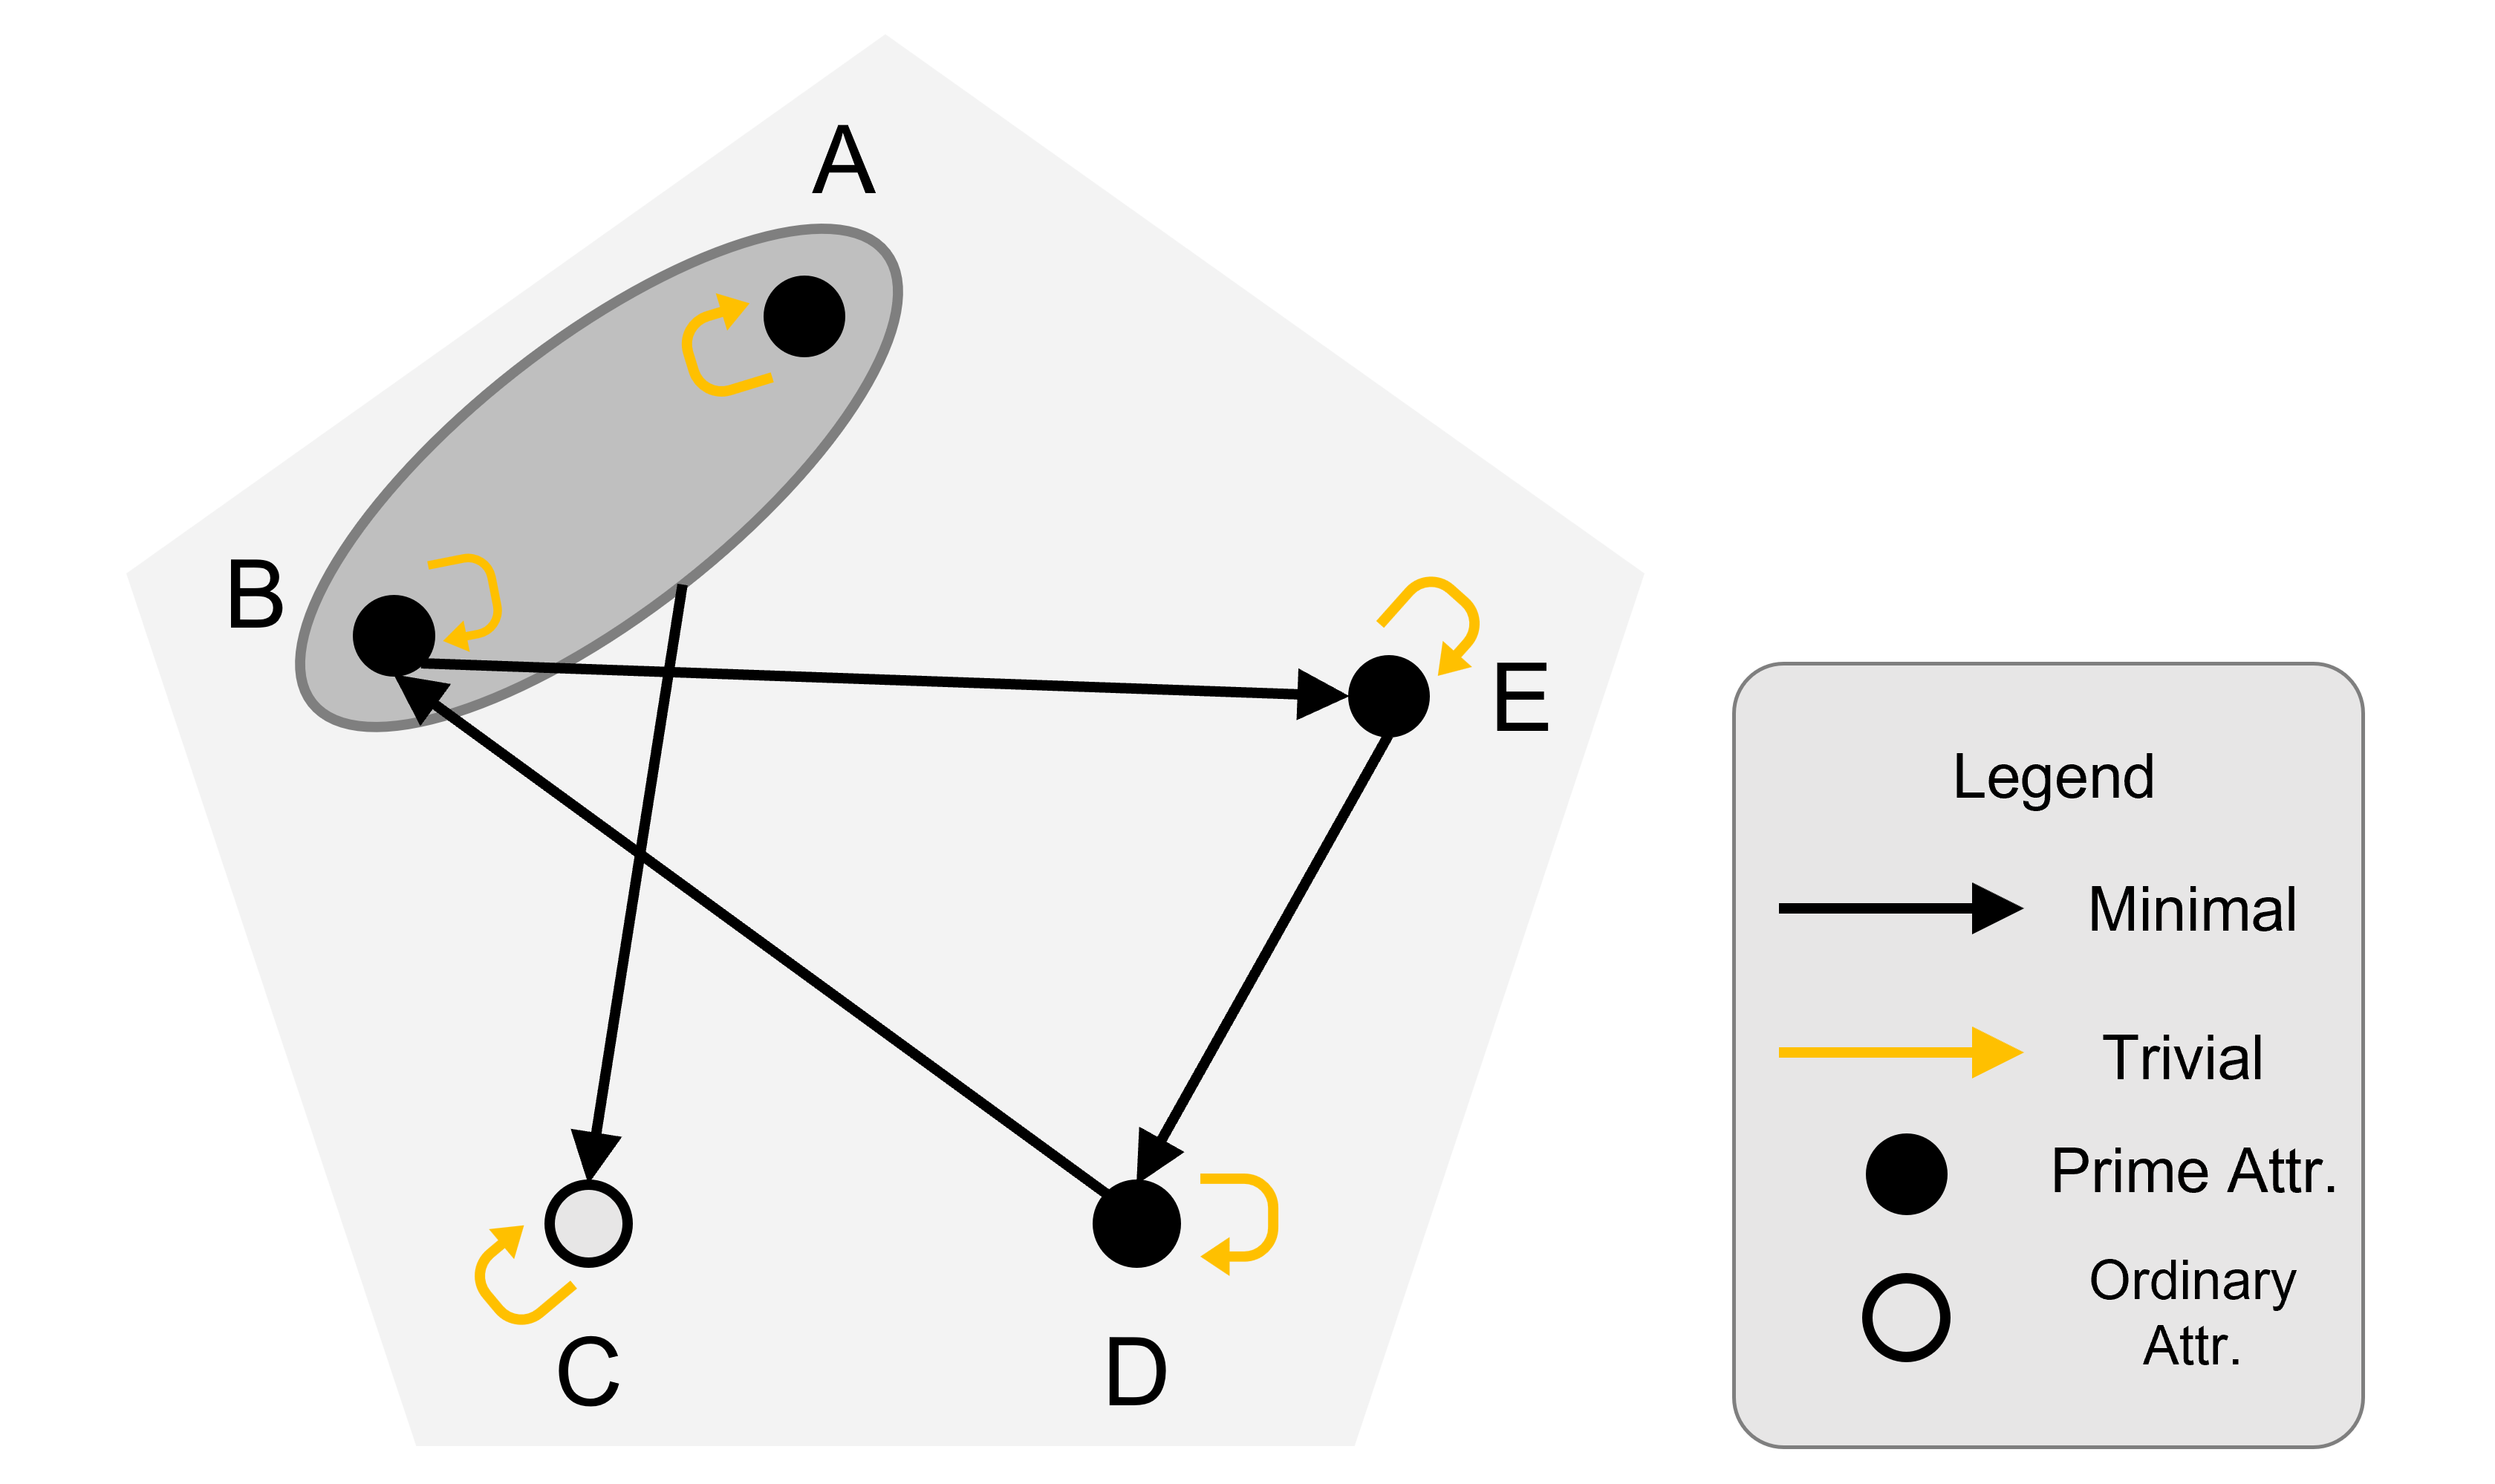
\includegraphics[width=0.85\textwidth, trim=0 0 0 0, clip]{4221-t3/images/q1.png}
	\end{figure}
\end{frame}

\begin{frame}[fragile]{Question 1 (a-b) Cont.}
	Now let's remove those information that is not essential from this closure:\\\vspace{3pt}
	We can remove from the RHS the members of the set on the LHS, as it also keeps all the essential information:\\\vspace{6pt}
	\begin{columns}[t]
		\column{0.45\textwidth}
		$\{A, B\}^{+}= \{C, D, E\}$\\
		$\{A, D\}^{+}= \{B, C, E\}$\\
		$\{A, E\}^{+}= \{B, C, D\}$\\
		$\{B\}^{+}= \{D, E\}$\\
		$\{D\}^{+}= \{B, E\}$\\
		$\{E\}^{+}= \{B, D\}$\\ 
		$\{B, C\}^{+}= \{D, E\}$\\
		$\{B, D\}^{+}= \{E\}$\\
		\column{0.45\textwidth}	
		$\{B, E\}^{+}= \{D\}$\\
		$\{C, D\}^{+}= \{B, E\}$\\
		$\{C, E\}^{+}= \{B, D\}$\\
		$\{D, E\}^{+}= \{B\}$\\
		$\{B, C, D\}^{+}= \{E\}$\\
		$\{B, C, E\}^{+}= \{D\}$\\
		$\{C, D, E\}^{+}= \{B\}$		
	\end{columns}
\end{frame}

\begin{frame}[fragile]{Question 1 (a-b) Cont.}
	Remark: We can even remove an equality if the LHS is a superset of another equality LHS and its RHS is a subset of the RHS (e.g., give $\{E\}^{+}= \{B, D\}$ and $\{C, D, E\}^{+}= \{B\}$, we can omit the second one). It also keeps all the essential information:\\\vspace{6pt}

	$\{A, B\}^{+}= \{C, D, E\}$\\
		$\{A, D\}^{+}= \{B, C, E\}$\\
		$\{A, E\}^{+}= \{B, C, D\}$\\
		$\{B\}^{+}= \{D, E\}$\\
		$\{D\}^{+}= \{B, E\}$\\
		$\{E\}^{+}= \{B, D\}$\\ \vspace{7pt}
	
	\textbf{(b) What are the candidate keys of $R$ with $\Sigma$?}\\ \vspace{3pt}
	The candidate keys are $\{A,B\}$, $\{A,D\}$ and $\{A,E\}$.\\
\end{frame}

\begin{frame}[fragile]{Question 1 (c) Minimal Cover}
	\textbf{(c) Find a minimal cover of $R$ with $\Sigma$ that can be reached from $\Sigma$ using the algorithm from the lecture.}\\ \vspace{5pt}
	\textbf{Solution}: Use the three step approach then you should be able to find one.\\\vspace{5pt}
	We start from $\Sigma$: \\\vspace{5pt}
	$\{A, B\} \rightarrow \{C\}$\\
	$\{D\} \rightarrow \{D, B\}$\\
	$\{B\} \rightarrow \{E\}$\\
	$\{E\} \rightarrow \{D\}$\\
	$\{A, B, D\} \rightarrow \{A, B, C, D\}$\\\vspace{5pt}
	\textbf{Step 1}, we simplify the right-hand sides to obtain $\Sigma'$:\\\vspace{3pt}
	\begin{columns}[t]
		\column{0.45\textwidth}
		$\{A, B\} \rightarrow \{C\}$\\
		\underline{$\{D\} \rightarrow \{D\}$}\\
		\underline{$\{D\} \rightarrow \{B\}$}\\
		$\{B\} \rightarrow \{E\}$\\
		$\{E\} \rightarrow \{D\}$\\
		\column{0.45\textwidth}
		\underline{$\{A, B, D\} \rightarrow \{A\}$}\\	
		\underline{$\{A, B, D\} \rightarrow \{B\}$}\\	
		\underline{$\{A, B, D\} \rightarrow \{C\}$}\\	
		\underline{$\{A, B, D\} \rightarrow \{D\}$}\\
	\end{columns}
\end{frame}

\begin{frame}[fragile]{Question 1 (c) Cont.}
	\textbf{Step 2}, we construct $\Sigma''$, which is equivalent to $\Sigma'$ (and to $\Sigma$), by minimizing the LHS of every functional dependency in $\Sigma'$. We may have the choice between several possible simplifications. We only need to choose one:\\\vspace{3pt}
	\begin{columns}[t]
		\column{0.23\textwidth}
		$\{A, B\} \rightarrow \{C\}$\\
		$\{D\} \rightarrow \{D\}$\\
		$\{D\} \rightarrow \{B\}$\\
		$\{B\} \rightarrow \{E\}$\\
		$\{E\} \rightarrow \{D\}$\\
		\column{0.7\textwidth}
		$\{A, \cancel{B, D}\} \rightarrow \{A\}$ because $\{A\} \rightarrow \{A\}$\\	
		$\{\cancel{A}, B, \cancel{D}\} \rightarrow \{B\}$ because $\{B\} \rightarrow \{B\}$\\	
		$\cancel{\{A, B, D\} \rightarrow \{C\}}$ because $\{A, B\} \rightarrow \{C\}$\\	
		$\{\cancel{A, B}, D\} \rightarrow \{D\}$because $\{D\} \rightarrow \{D\}$\\
	\end{columns}
\end{frame}

\begin{frame}[fragile]{Question 1 (c) Cont.}
	\textbf{Step 3}, we construct $\Sigma'''$, which is equivalent to $\Sigma''$ (and to $\Sigma$), by minimizing the whole set $\Sigma''$ (e.g., removing trivial ones). We may have the choice between several possible simplifications. The choice depends on the order in which we consider the functional dependency:\\\vspace{3pt}
	$\{A, B\} \rightarrow \{C\}$\\
	$\cancel{\{D\} \rightarrow \{D\}}$ because it is trivial.\\
	$\{D\} \rightarrow \{B\}$\\
	$\{B\} \rightarrow \{E\}$\\
	$\{E\} \rightarrow \{D\}$\\\vspace{3pt}
	
	\textbf{The (not unique) result is:} \\\vspace{3pt}
	$\Sigma'''=\{\{A, B\} \rightarrow \{C\}, \{D\} \rightarrow \{B\}, \{B\} \rightarrow \{E\}, \{E\} \rightarrow \{D\}\}$
	\\\vspace{5pt}
	\textcolor{red}{\textbf{NOTES FROM TA:} There is another minimal cover can be derived by this 3-step method, with the order of dependency reshuffled. You may download and refer to the Luminus files (Tutorials/Dependency/Tutorial Dependency (some answers).pdf) for more details.\\Both minimal cover are so called ``reachable with the algorithm''.} 
\end{frame}

\begin{frame}[fragile]{Question 1 (d) Minimal Cover}
	\textbf{(d) Find all the minimal covers of $R$ with $\Sigma$}\\ \vspace{5pt}
	\textbf{Solution}: There are \textbf{15} different minimal covers.\\\vspace{2pt}
	{\footnotesize
	(1)  $\Sigma'''=\{\{A, B\} \rightarrow \{C\}, \{D\} \rightarrow \{B\}, \{B\} \rightarrow \{E\}, \{E\} \rightarrow \{D\}\}$ \\\vspace{2pt}
	(2)  $\Sigma'''=\{\{A, B\} \rightarrow \{C\}, \{B\} \rightarrow \{D\}, \{E\} \rightarrow \{B\}, \{D\} \rightarrow \{E\}\}$ \\\vspace{2pt}
	(3)  $\Sigma'''=\{\{A, B\} \rightarrow \{C\}, \{B\} \rightarrow \{D\}, \{D\} \rightarrow \{B\}, \{B\} \rightarrow \{E\}, \{E\} \rightarrow \{B\}\}$ \\\vspace{2pt}
	(4)  $\Sigma'''=\{\{A, B\} \rightarrow \{C\}, \{B\} \rightarrow \{D\}, \{D\} \rightarrow \{B\}, \{E\} \rightarrow \{D\}, \{D\} \rightarrow \{E\}\}$ \\\vspace{2pt}
	(5)  $\Sigma'''=\{\{A, B\} \rightarrow \{C\}, \{E\} \rightarrow \{B\}, \{B\} \rightarrow \{E\}, \{E\} \rightarrow \{D\}, \{D\} \rightarrow \{E\}\}$ \\\vspace{2pt}
	
	(6)  $\Sigma'''=\{\{A, D\} \rightarrow \{C\}, \{D\} \rightarrow \{B\}, \{B\} \rightarrow \{E\}, \{E\} \rightarrow \{D\}\}$ \\\vspace{2pt}
	(7)  $\Sigma'''=\{\{A, D\} \rightarrow \{C\}, \{B\} \rightarrow \{D\}, \{E\} \rightarrow \{B\}, \{D\} \rightarrow \{E\}\}$ \\\vspace{2pt}
	(8)  $\Sigma'''=\{\{A, D\} \rightarrow \{C\}, \{B\} \rightarrow \{D\}, \{D\} \rightarrow \{B\}, \{B\} \rightarrow \{E\}, \{E\} \rightarrow \{B\}\}$ \\\vspace{2pt}
	(9)  $\Sigma'''=\{\{A, D\} \rightarrow \{C\}, \{B\} \rightarrow \{D\}, \{D\} \rightarrow \{B\}, \{E\} \rightarrow \{D\}, \{D\} \rightarrow \{E\}\}$ \\\vspace{2pt}
	(10) $\Sigma'''=\{\{A, D\} \rightarrow \{C\}, \{E\} \rightarrow \{B\}, \{B\} \rightarrow \{E\}, \{E\} \rightarrow \{D\}, \{D\} \rightarrow \{E\}\}$ \\\vspace{2pt}
	
	(11) $\Sigma'''=\{\{A, E\} \rightarrow \{C\}, \{D\} \rightarrow \{B\}, \{B\} \rightarrow \{E\}, \{E\} \rightarrow \{D\}\}$ \\\vspace{2pt}
	(12) $\Sigma'''=\{\{A, E\} \rightarrow \{C\}, \{B\} \rightarrow \{D\}, \{E\} \rightarrow \{B\}, \{D\} \rightarrow \{E\}\}$ \\\vspace{2pt}
	(13) $\Sigma'''=\{\{A, E\} \rightarrow \{C\}, \{B\} \rightarrow \{D\}, \{D\} \rightarrow \{B\}, \{B\} \rightarrow \{E\}, \{E\} \rightarrow \{B\}\}$ \\\vspace{2pt}
	(14) $\Sigma'''=\{\{A, E\} \rightarrow \{C\}, \{B\} \rightarrow \{D\}, \{D\} \rightarrow \{B\}, \{E\} \rightarrow \{D\}, \{D\} \rightarrow \{E\}\}$ \\\vspace{2pt}
	(15) $\Sigma'''=\{\{A, E\} \rightarrow \{C\}, \{E\} \rightarrow \{B\}, \{B\} \rightarrow \{E\}, \{E\} \rightarrow \{D\}, \{D\} \rightarrow \{E\}\}$ \\\vspace{2pt}
	}
\end{frame}

\begin{frame}[fragile]{Question 1 (d) Minimal Cover}
	{\small\textcolor{red}{\textbf{NOTES FROM TA:} These 15 minimal covers contains those cannot be obtained (aka. not reachable) through the 3-step method. You may design your algorithm to look into the \textbf{closure} ($\Sigma^{+}$) rather than the original $\Sigma$ to find all of them.}} \\
	You may confuse at the first glance. But don't worry, it's easy :D\\\vspace{2pt}
	Let's look at the first 5 minimal covers, with the visualization of $\Sigma$ as the reference:\\\vspace{3pt}
	{\footnotesize
		$\Sigma'''=\{\{A, B\} \rightarrow \{C\}, \{D\} \rightarrow \{B\}, \{B\} \rightarrow \{E\}, \{E\} \rightarrow \{D\}\}$ \\\vspace{2pt}
		$\Sigma'''=\{\{A, B\} \rightarrow \{C\}, \{B\} \rightarrow \{D\}, \{E\} \rightarrow \{B\}, \{D\} \rightarrow \{E\}\}$ \\\vspace{4pt}
		$\Sigma'''=\{\{A, B\} \rightarrow \{C\}, \textcolor{red}{\{B\} \rightarrow \{D\}, \{D\} \rightarrow \{B\}}, \textcolor{blue}{\{B\} \rightarrow \{E\}, \{E\} \rightarrow \{B\}}\}$ \\\vspace{2pt}
		$\Sigma'''=\{\{A, B\} \rightarrow \{C\}, \textcolor{red}{\{B\} \rightarrow \{D\}, \{D\} \rightarrow \{B\}}, \textcolor{brown}{\{E\} \rightarrow \{D\}, \{D\} \rightarrow \{E\}}\}$ \\\vspace{2pt}
		$\Sigma'''=\{\{A, B\} \rightarrow \{C\}, \textcolor{blue}{\{B\} \rightarrow \{E\}, \{E\} \rightarrow \{B\}}, \textcolor{brown}{\{E\} \rightarrow \{D\}, \{D\} \rightarrow \{E\}}\}$ \\\vspace{2pt}
	}
	\vspace{5pt}
	\begin{columns}[t]
		\column{0.4\textwidth}
	\begin{figure}
		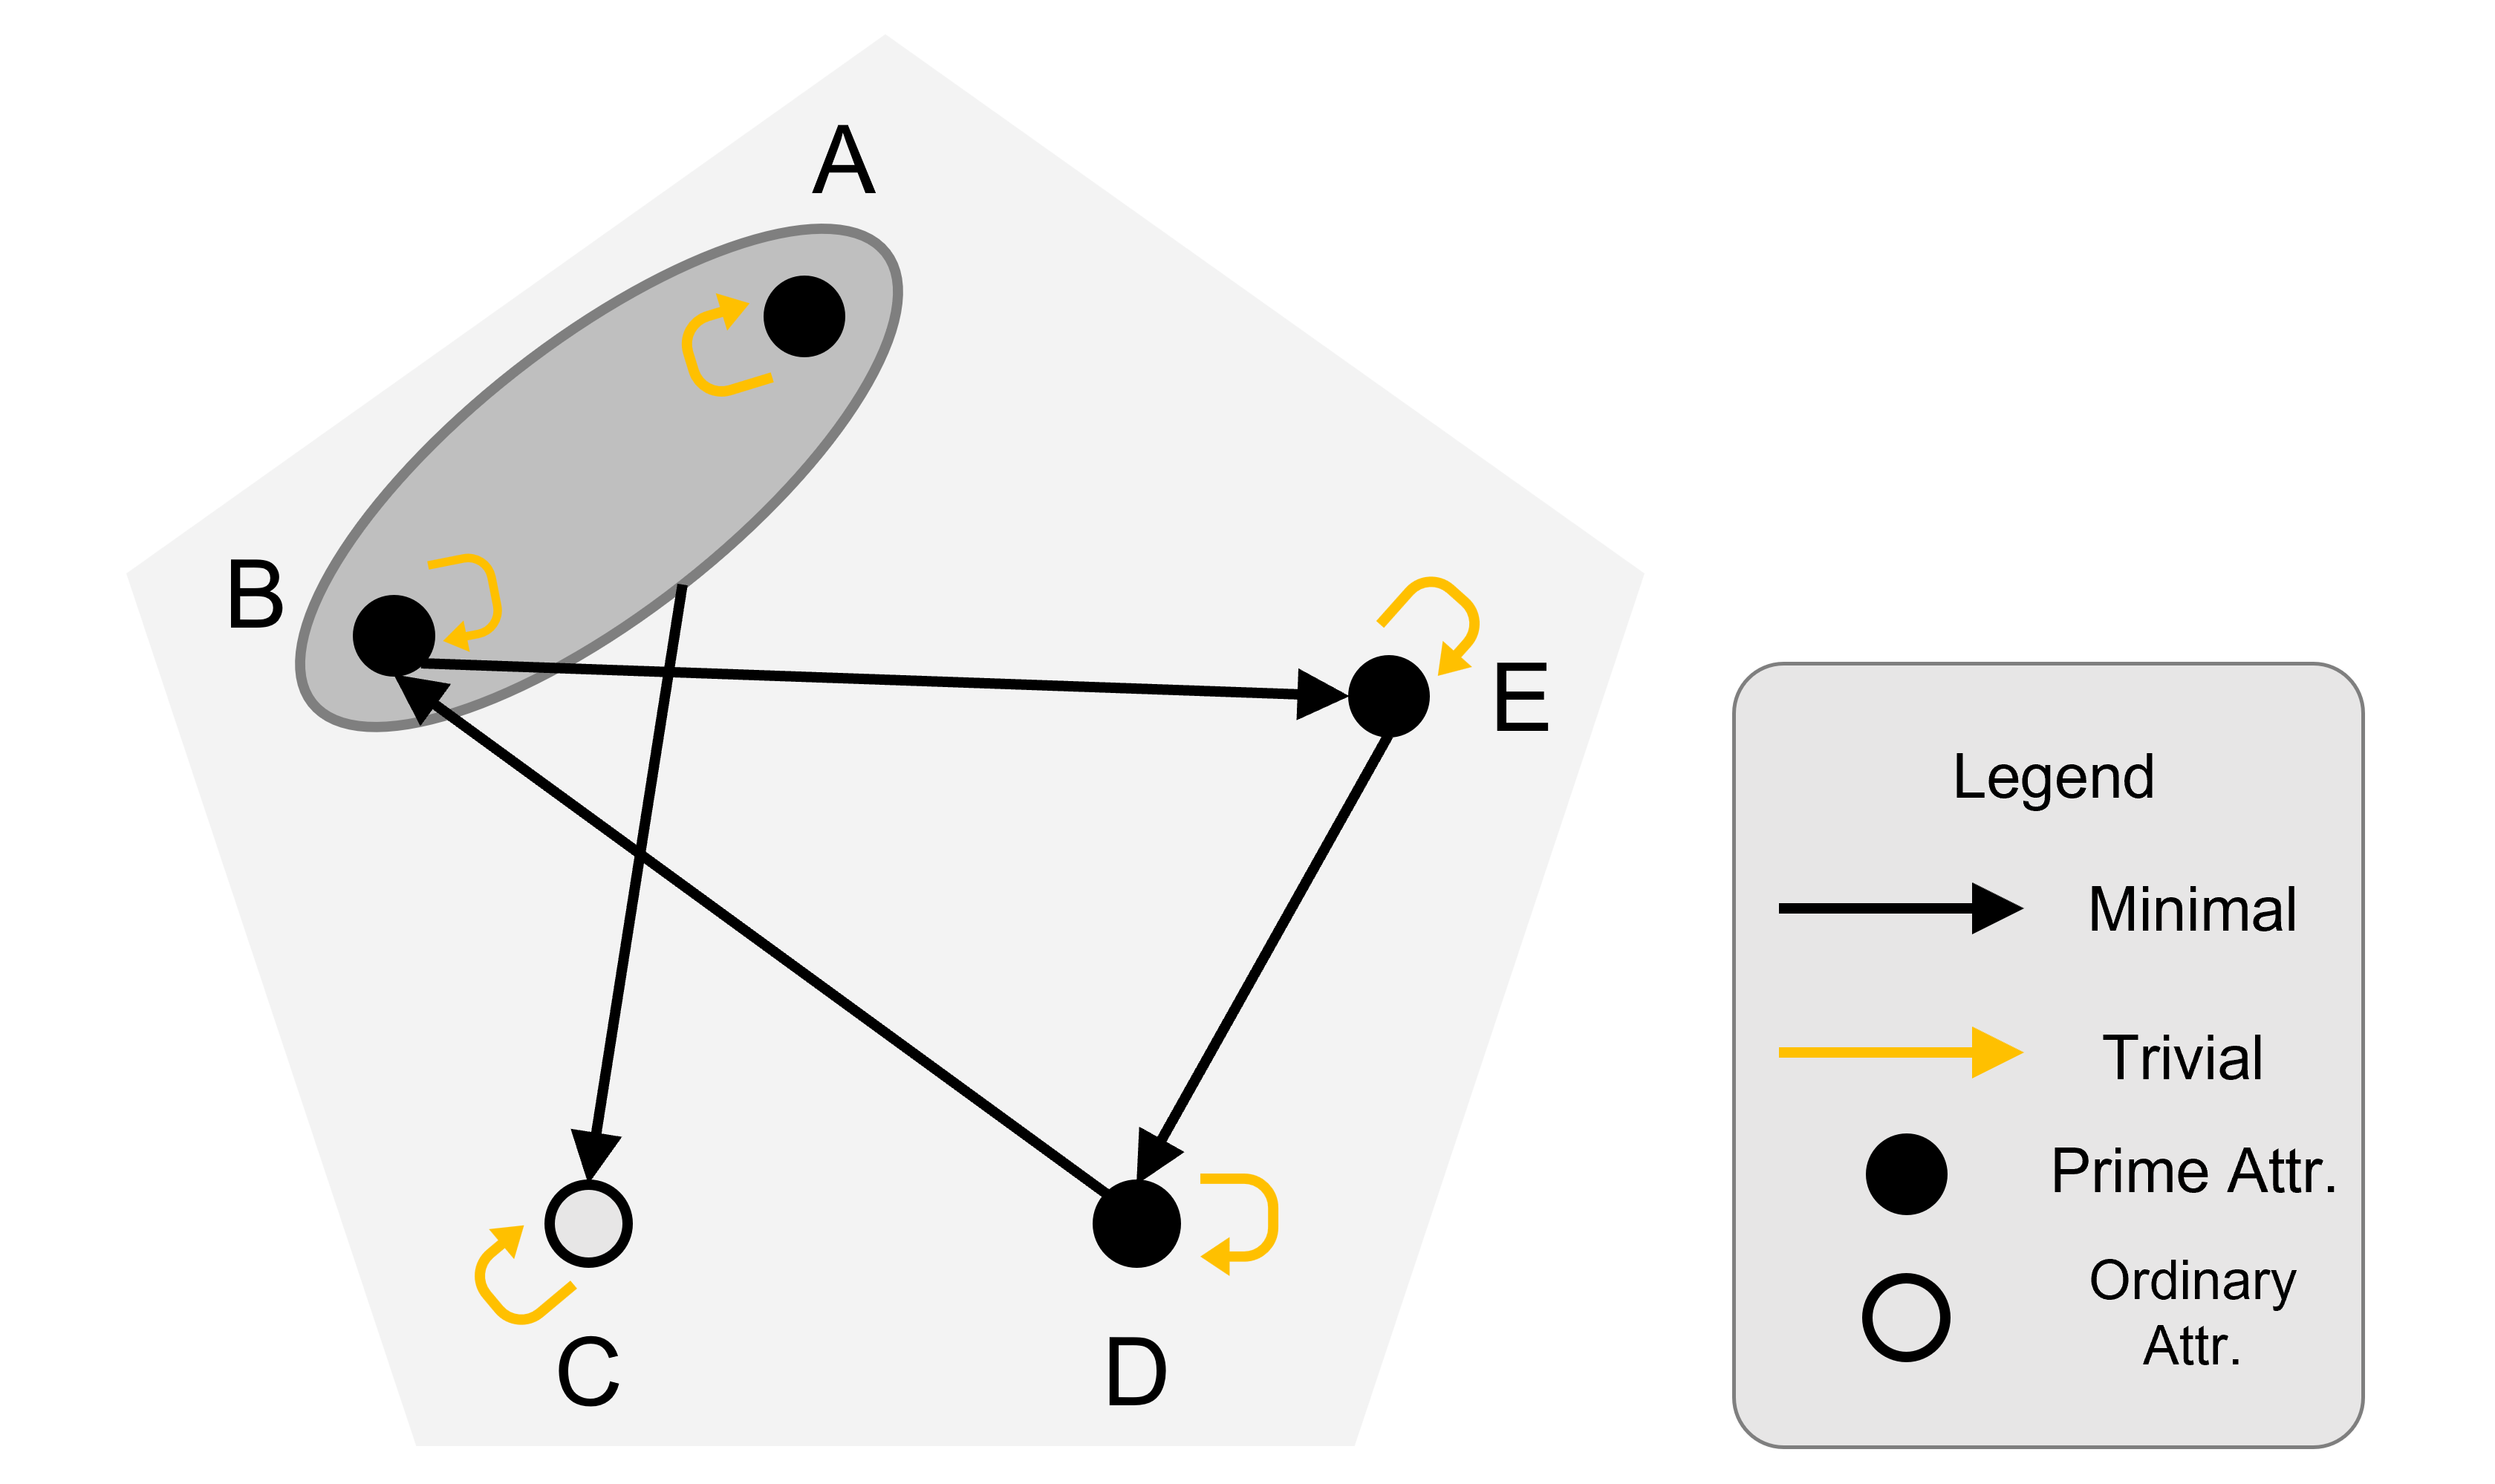
\includegraphics[width=0.75\textwidth, trim=0 0 0 0, clip]{4221-t3/images/q1.png}
	\end{figure}

	\column{0.55\textwidth}
	{\small
	We find for each $\{??\} \rightarrow \{C\}$, there are \textbf{five} legal minimal covers. \\\vspace{2pt}
	Then we know there are \textbf{three} $\{??\} \rightarrow \{C\}$ possible $\{??\} \rightarrow \{C\}$.\\\vspace{2pt}
	Thus there exists $3\times 5=15$ different minimal covers. 
	}
\end{columns}
\end{frame}

\begin{frame}[fragile]{Question 1 (e) Armstrong Axioms}
	\textbf{(e) Prove, using the three Armstrong axioms, that the following set of functional dependencies is equivalent to $\Sigma$.} \\\vspace{5pt}
	$\Sigma''''=\{\{A, B\} \rightarrow \{C, D, E\}, \{A, D\} \rightarrow \{B, C, E\}, \{A, E\} \rightarrow \{B, C, D\}, \{B\} \rightarrow \{D, E\}, \{D\} \rightarrow \{B, E\}, \{E\} \rightarrow \{B, D\}\}$.\\\vspace{5pt}
	
	\textbf{Solution}: We prove that every functional dependency in one of $\Sigma$ and $\Sigma''''$ can obtained from those in the other set.\\\vspace{2pt}
	For example $\{B\} \rightarrow \{D,E\}$ can be obtained from $\Sigma$.
	
	\begin{enumerate}
		\item We know that $\{B\} \rightarrow \{E\}$.
		\item We know that $\{E\} \rightarrow \{D\}$.
		\item Therefore we have $\{E\} \rightarrow \{D, E\}$ by Augmentation of (2) with $\{E\}$.
		\item Therefore we have $\{B\} \rightarrow \{D, E\}$ by Transitivity of (1) and (3).
	\end{enumerate}

	Q.E.D.\\\vspace{7pt}
	
	\textit{In fact you can prove by change (3) to:}\\
	Therefore we have $\{B\} \rightarrow \{D\}$ by by Transitivity of (1) and (2).\\ 
	Then we have $\{B\} \rightarrow \{D, E\}$ by Augmentation of (3) with (1).
\end{frame}


\begin{frame}{}
	\centering  
	For any further question, please feel free to email me:\vspace{10pt}
	
	huasong.meng@u.nus.edu\\\vspace{3pt}
	% Or you can whatsapp/wechat me via: 81028639 \vspace{20pt}
	
	\begin{tcolorbox}
		\begin{center}
			\textcolor{red}{Copyright 2021 Mark H. Meng. All rights reserved.}
		\end{center}
	\end{tcolorbox}
\end{frame}